\documentclass[../../main.tex]{subfiles}

%This section of the proposal is used to assess the adequacy of the resources available to perform the effort proposed to satisfy both the Intellectual Merit and Broader Impacts review criteria. Proposers should describe only those resources that are directly applicable. Proposers should include an aggregated description of the internal and external resources (both physical and personnel) that the organization and its collaborators, and subawardees will provide to the project, should it be funded. Such information must be provided in this section, in lieu of other parts of the proposal (e.g., Budget Justification, Project Description). The description should be narrative in nature and must not include any quantifiable financial information.
 
\begin{document}
\label{sec:fac_equip_res}

\begin{figure}[hb]
\centering
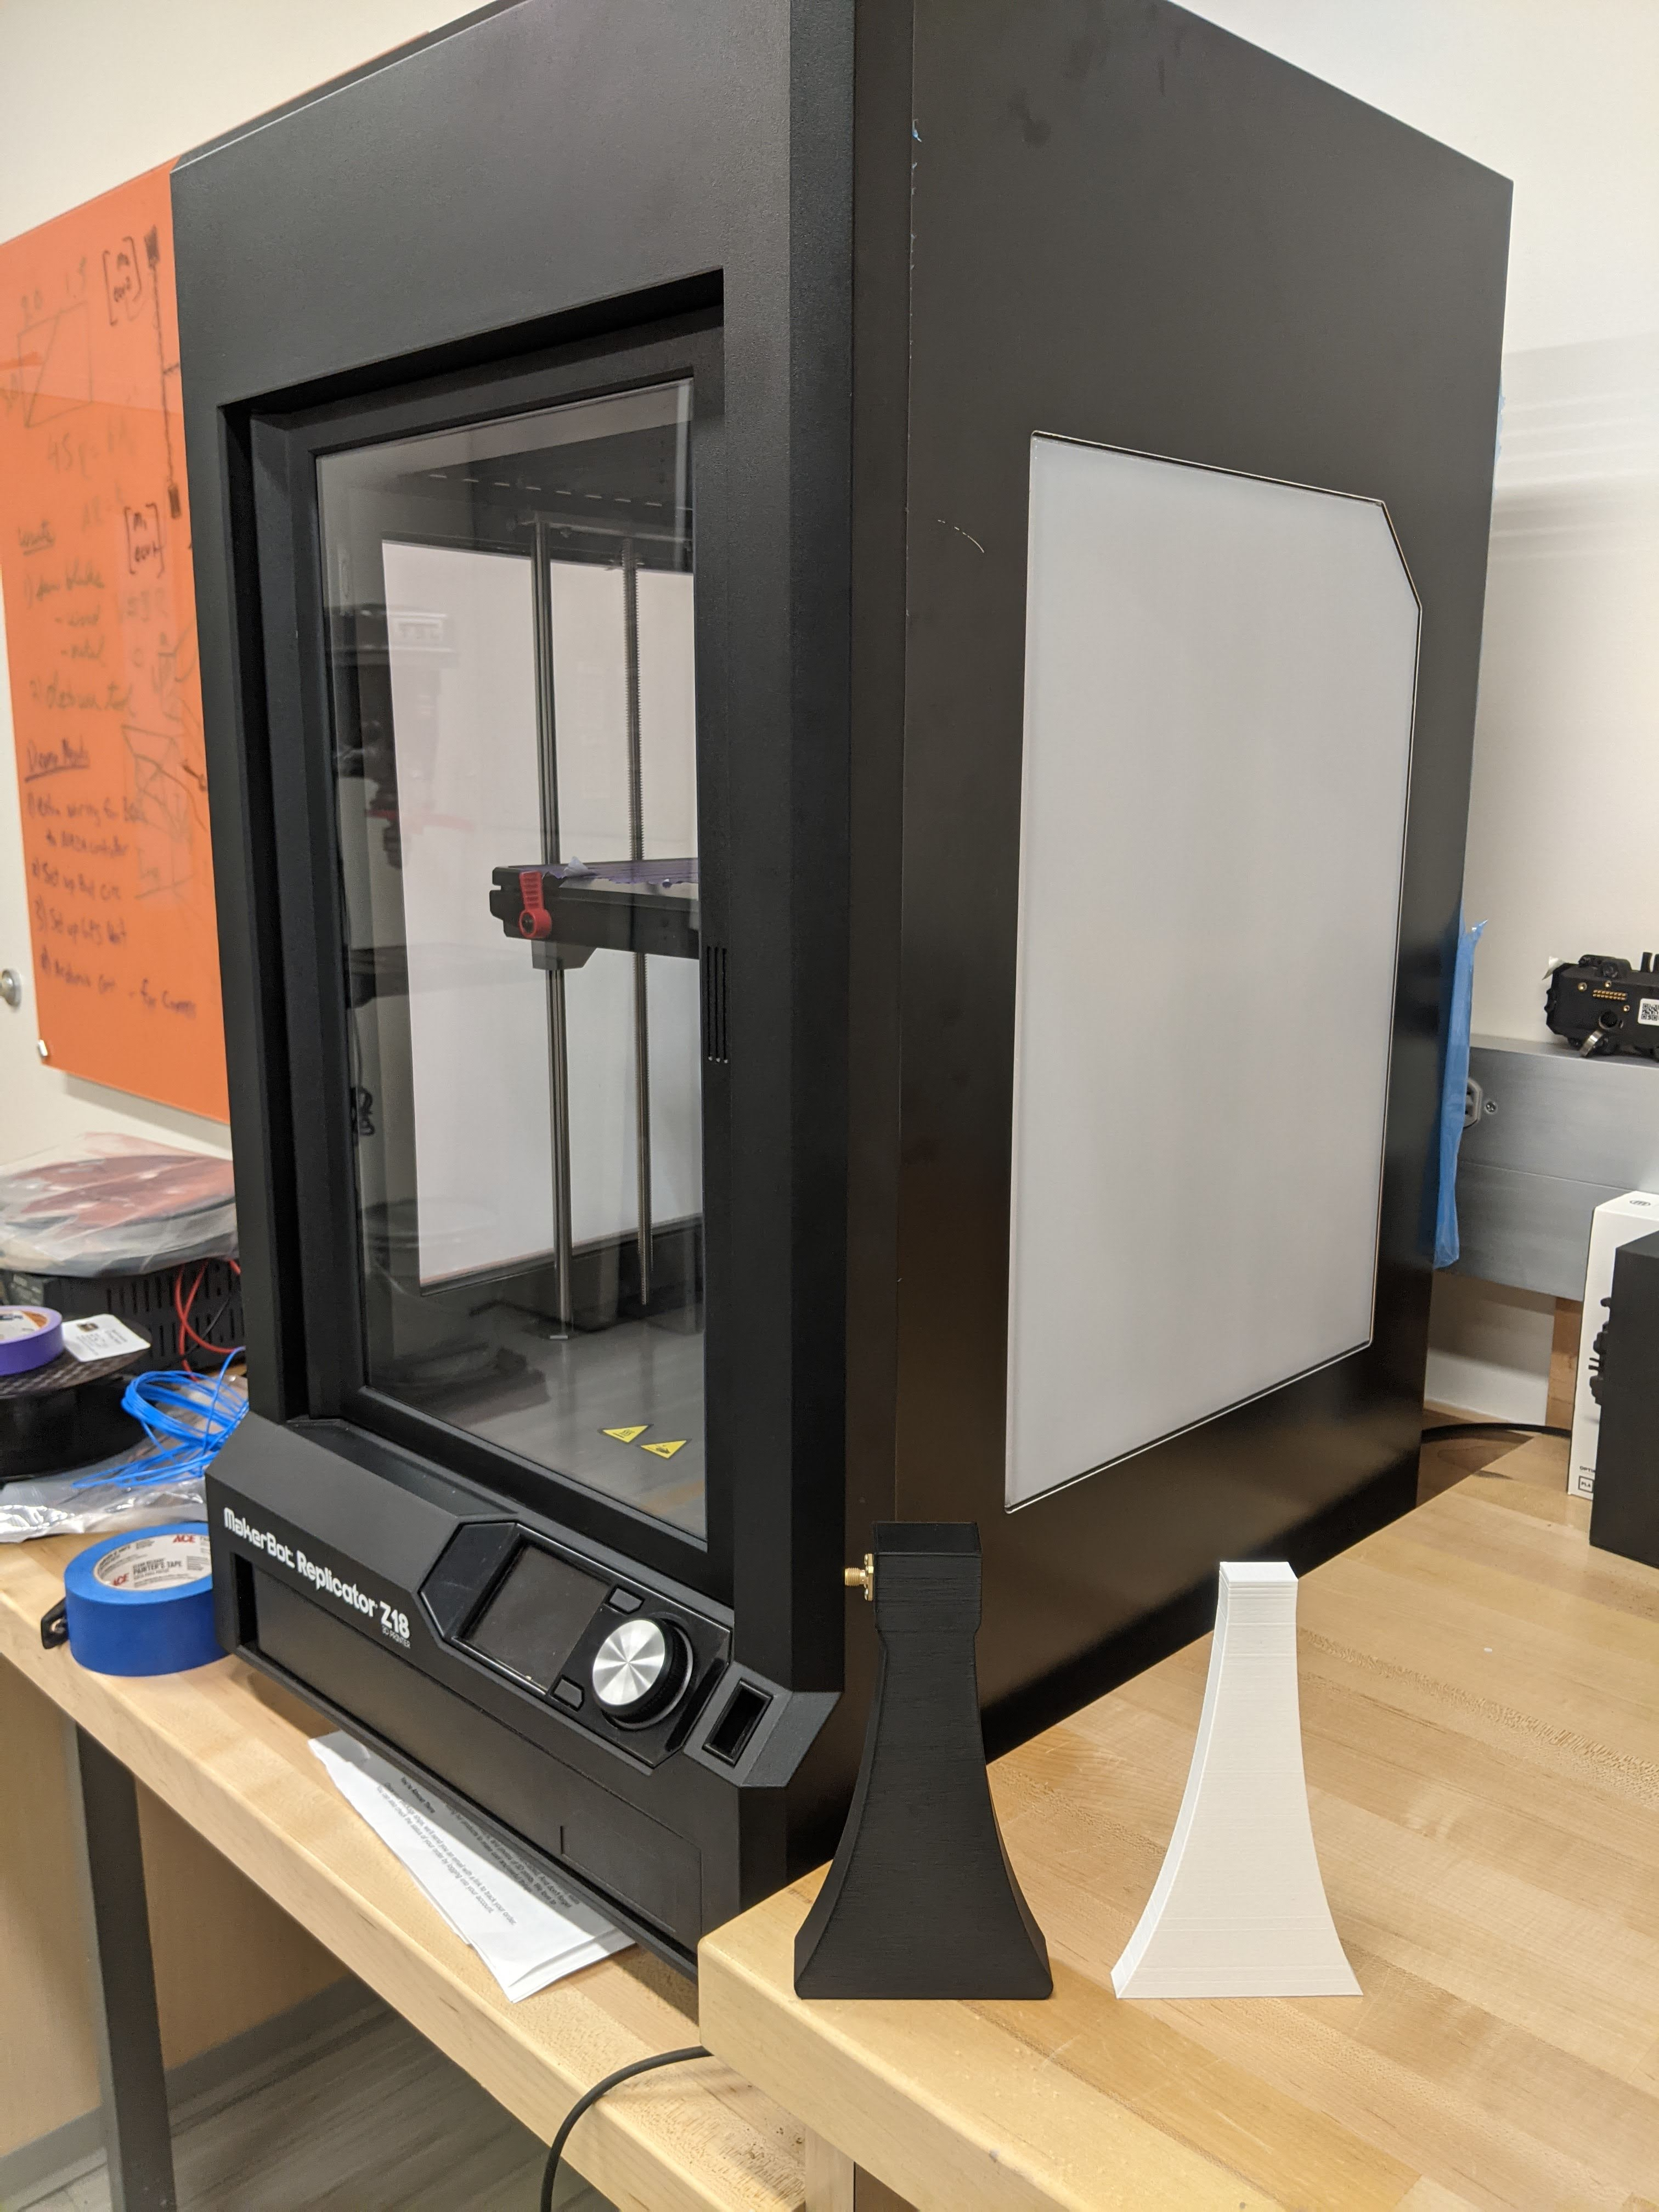
\includegraphics[width=0.2\textwidth]{figures/3dprinter.jpg}
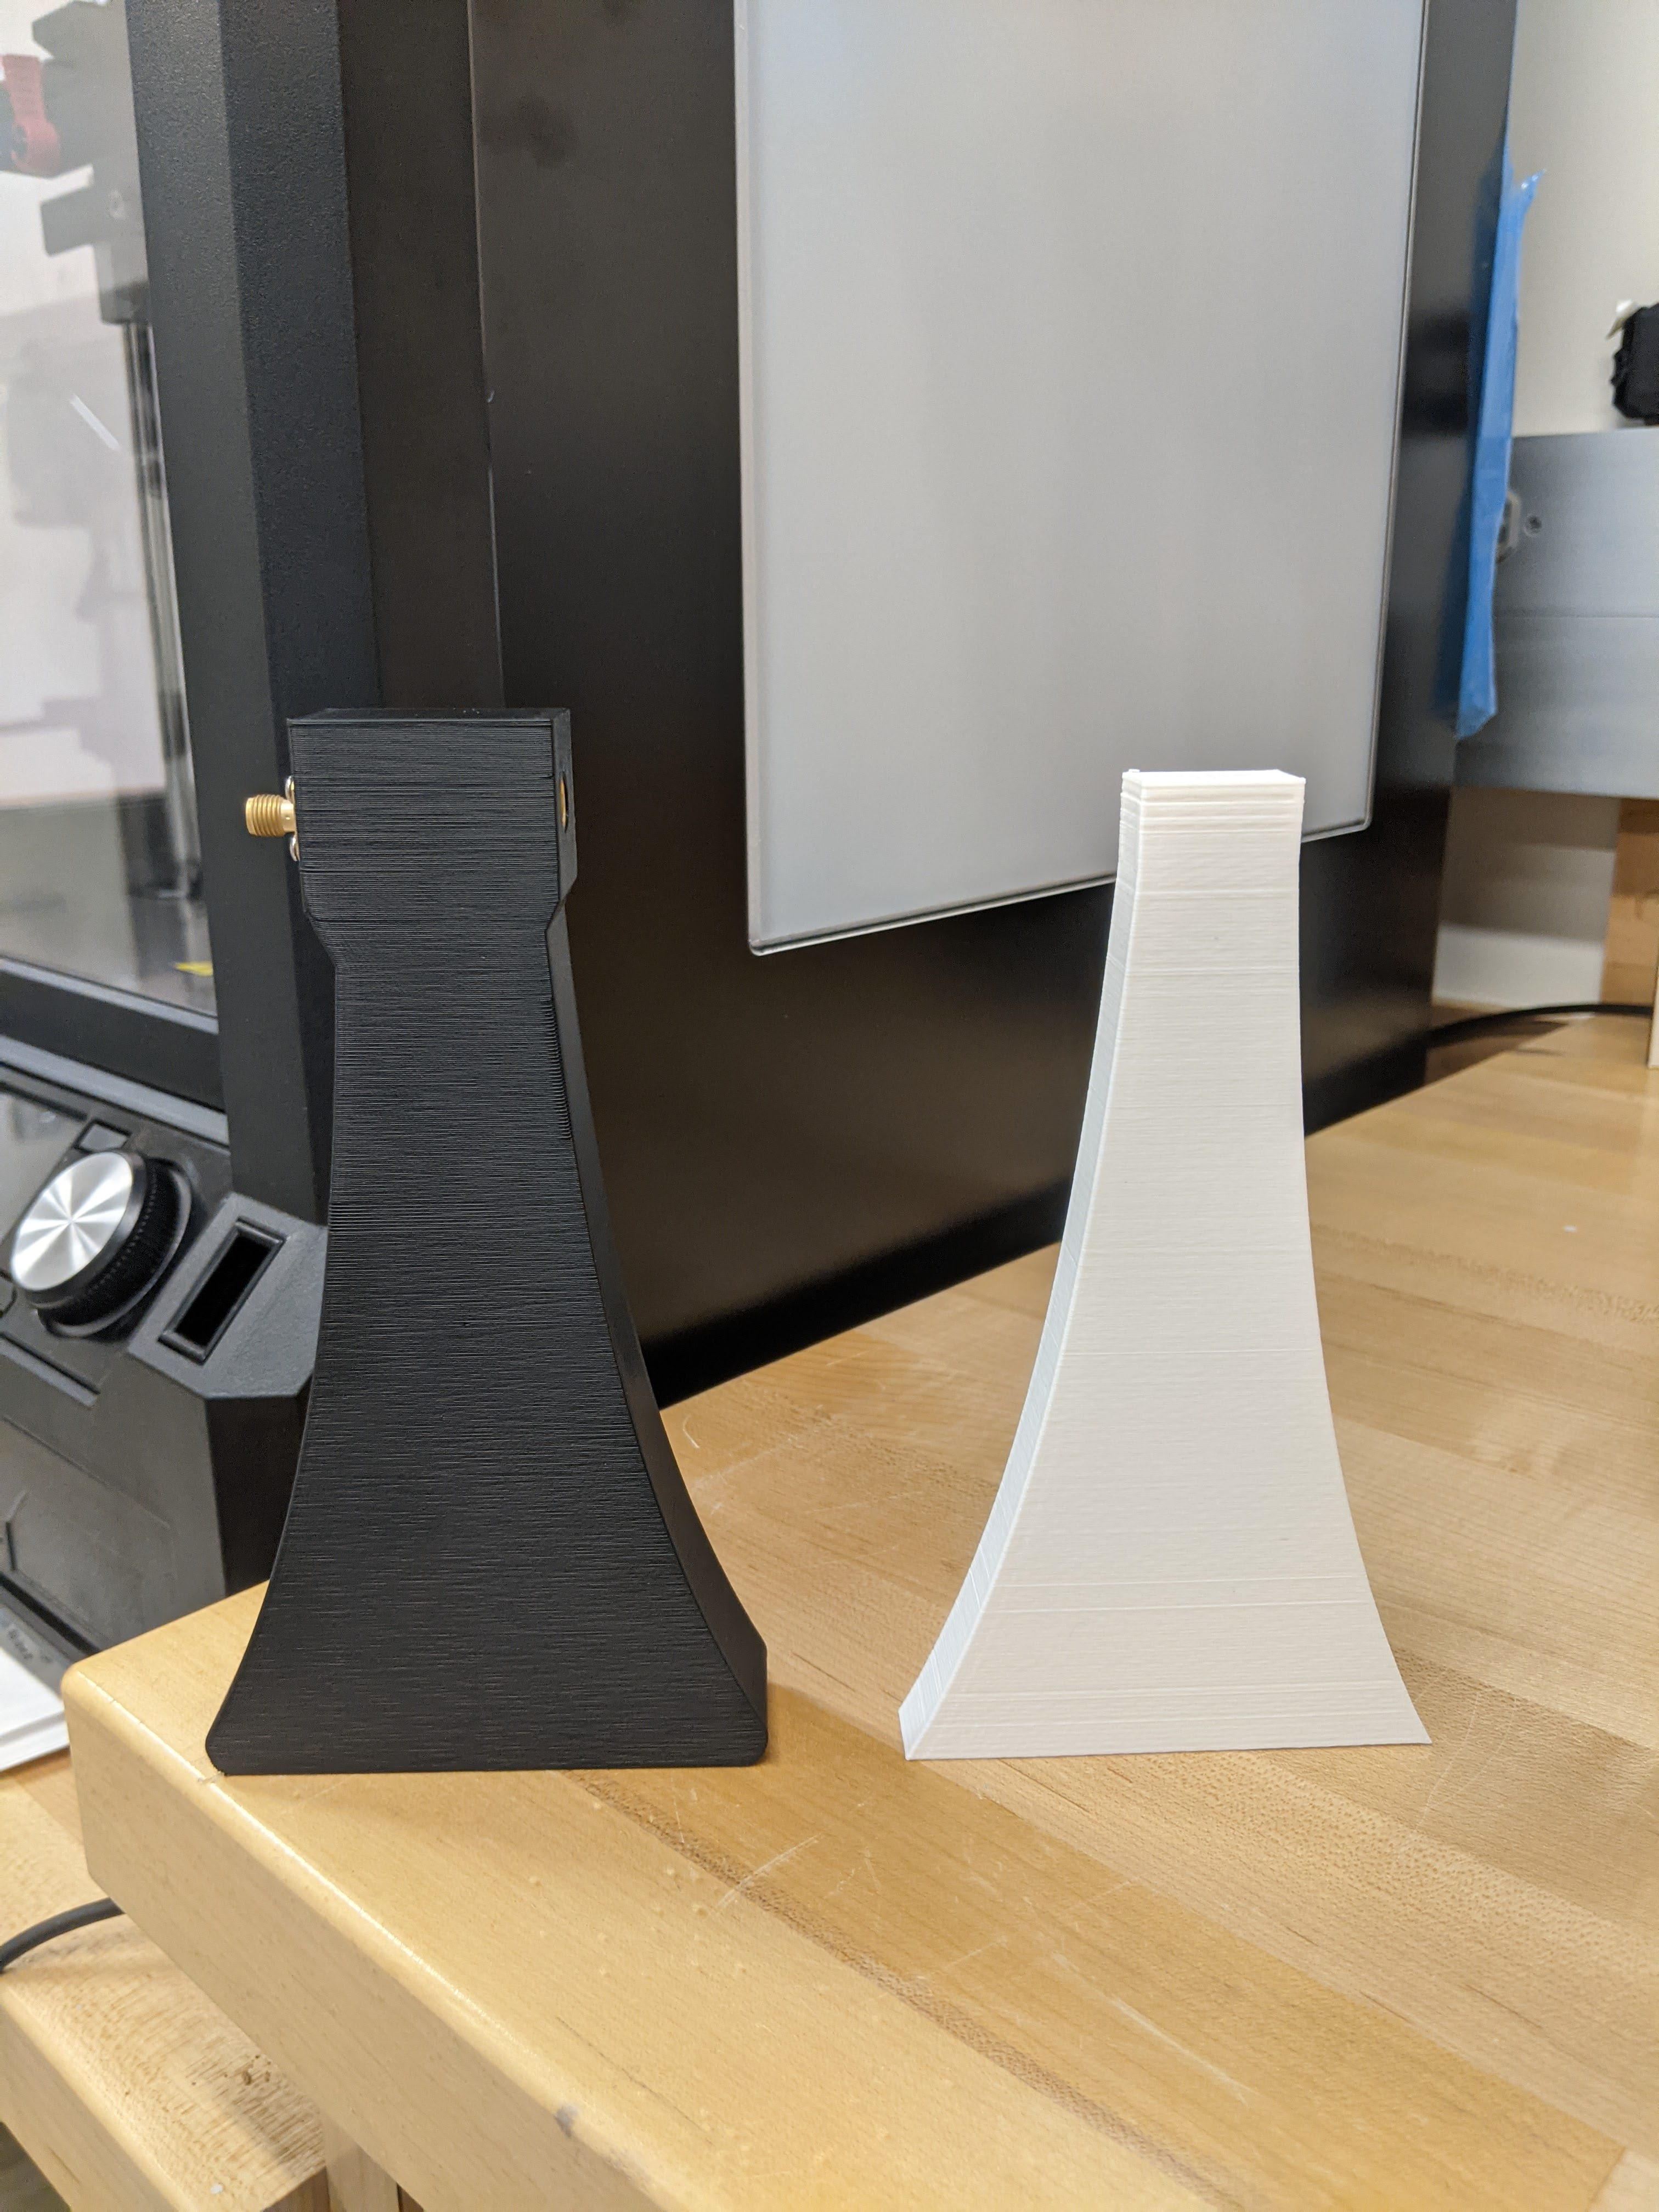
\includegraphics[width=0.2\textwidth]{figures/3dprinter_2.jpg}
\caption{\label{fig:3d_print_fac} (Left) MakerBot 3D printer, with PLA horn model (white), and  proto-pasta with SMA connector (black). (Right) Close-up of horns.}
\end{figure}


In Summer 2022, we received a third ONR fellowship focusing on GPS modernization\footnote{ONR regulations state that a gap year is required.  For our group, Senior Fellowship eligibility begins in Summer 2024.}.  Alongside this work, we continued to refine the open-source CEM results.  We learned to simulate the full 3D horns stored in CAD files using parallel processing, achieving an order of magnitude reduction in computation time.  The results are shown in Fig. \ref{fig:3d_cad}.  In Fig. \ref{fig:3d_cad} (a), the main lobes are designed to point to 0 degrees (x-direction) for the E-plane (x-y plane), and 90 degrees for the H-plane (x-z plane).  The E-plane contains the linearly polarized radiation vector.  In Fig. \ref{fig:3d_cad} (b), the voltage standing wave ratio (VSWR) is shown.  The VSWR is a common figure of merit for RF antennas, related to the S-parameters.  The VSWR approaches 1 for an efficiently radiating antenna, and infinity for no efficiency.  The radiation patterns match expectations for horn antennas (see Fig. 19 of \cite{8786183}).  The VSWR results demonstrate efficient radiation in the bandwidth [0.5 - 6] GHz.  We presented our progress at the annual MeepCon 2022 at the Massachusetts Institute of Technology (MIT) \cite{meepcon2022}.  We learned new techniques for integrating MEEP and machine learning tools \cite{meepcon2022_2}, and how eager MEEP developers are to collaborate in the RF regime.  \\ \vspace{2.5mm}

\subsection{RF Laboratory Capability and Prior ONR Funding}

We are required to take a research gap year in Summer 2023, according to ONR regulations.  However, we have now begun an Educational Partnership Agreement (EPA) between NSWC Corona and Whittier College.  NSWC Corona now has the ability to transfer laboratory equipment to Whittier College.  NSWC Corona has provided RF bench testing equipment that is perfectly suited to the proposed work.  A list of instruments transferred from NSWC Corona between 2020 and 2023 is shown in Tab. \ref{tab:equip}.  Our network analyzer and power sensors can perform S-parameter measurements over [9 kHz - 6 GHz] for our antennas under test (AUT).  Our signal generator can create calibration signals for our calibration antennas and AUT over [250 kHz - 6 GHz].  Our calibration antennas serve as benchmark devices for comparison to our 3D printed AUT.  Due to the precision and wide bandwith of these devices, regular calibration is required.  Our calibration kits serve this purpose.  Our laboratory is therefore well-equipped to complete the proposed work, and this minimizes budgetary impact. \\ \vspace{2.5mm}

This research has been completed with significant contributions from diverse undergraduate students.  We provide a summary of funding for personnel that have contributed to the early stages of this work in Tab. \ref{tab:funds}.  These researchers have diverse majors and interests, including our 3-2 Engineering Program (Wildanger), Physics and Math double major (Hartig), and Math/Integrated Computer Science (G\'{o}mez-Reed and Householder), and Physics and Astronomy (Goodman and Smith).   After Whittier College, these students have begun science and engineering roles that include the Laser Interferometer Gravitational-Wave Observatory (LIGO), the University of Southern California (USC), and The Aerospace Corporation.  Whittier College has a good track record of providing access to higher education, and careers in science and technology, to diverse students from Los Angeles County and beyond. \\ \vspace{2.5mm}

\begin{table}
\centering
\begin{tabular}{c c c}
Equipment & Bandwidth & Cost \\ \hline
Rohde and Schwartz ZVL6 Network Analyzer & 9 kHz to 6 GHz & \$20k \\
Rohde and Schwartz NRP-91 Power Sensors (2) & 9 kHz to 6 GHz & \$8k \\
Aeroflex 3416 Digital RF Signal Generator & 250kHz to 6 GHz & \$12k \\
Calibration antenna kits (2) & Varies by antenna & \$2k \\
Calibration test kits for Network Analyzer (2) & 6 kHz to 9 GHz & \$6k
\end{tabular}
\caption{\label{tab:equip} A listing of the equipment provided to our labs by the Office of Naval Research.}
\end{table}

\begin{table}
\centering
\begin{tabular}{c c c c}
Student/Professor & Grant Opportunity & Amount & Dates \\ \hline
Jordan C. Hanson & ONR Summer Faculty Fellow & \$16.5k & Summer 2022 \\
Dane Goodman & Summer researcher & Course credit & Summer 2022 \\
Andrew Householder & Summer researcher & Course credit & Summer 2022 \\
Raymond Hartig & Ondrasik-Groce Fellowship & \$5k & Summer 2022 \\
Jordan C. Hanson & ONR Summer Faculty Fellow & \$16.5k & Summer 2021 \\
Adam Wildanger & Fletcher Jones Fellowship & \$5k & Summer 2021 \\
Jordan C. Hanson & ONR Summer Faculty Fellow & \$16.5k & Summer 2020 \\
Raymond Hartig & Fletcher Jones Fellowship & \$5k & Summer 2020 \\
John Paul G\'{o}mez-Reed & Ondrasik-Groce Fellowship & \$7.5k & Summer-Fall 2019 \\
John Paul G\'{o}mez-Reed & Keck Fellowship & \$5k & Summer 2018 \\
Cassady Smith & Keck Fellowship & \$5k & Summer 2018 \\
\end{tabular}
\caption{\label{tab:funds} A listing of the grant opportunities awarded to our group for RF design, softrware development, and machine-learning.  All students are at the undergraduate level.}
\end{table}

\end{document}
